\documentclass{article}
\usepackage[utf8]{inputenc}
\usepackage{graphicx}
\usepackage{verbatim}
\usepackage{hyperref}
\usepackage{caption}
\graphicspath{ {/Users/brendan/Dropbox/JBParallel/} }


\title{CS207 Final Project: JBParallel}
\author{Jonah Kallenbach and Brendan Bozorgmir
\\jkallenbach@college.harvard.edu and bbozorgmir@college.harvard.edu}
\date{December 15, 2014}

\begin{document}

\maketitle

\textbf{ALL CODE IS HERE:} \url{https://github.com/jonahkall/JBParallel}

\section{Intro, Setup and Installation}

Our goal for this project was to implement a relatively simply but easily usable and fast library for parallelizing code.  Until the very end of the project, we did not look at any parallel libraries, including OpenMP: at Cris's recommendation, we wanted to learn by implementing everything ourselves.  The end result, thousands of lines of code and dozens of hours testing later is a success: we have sped up tons of code and had a lot of fun thinking and implementing algorithms in parallel, and other people, we hear, are using our library.  In fact, by sacrificing a bit of generality, we were able to make our code faster than OpenMPs own functions (e.g. omp parallel for)!

We will first provide a quick guide to using our software on one's own computer.  We tried to make the interface as simple and useful as possible.
 
\paragraph*{Determine if your problem can be parallelized.}
\begin{itemize}
\item{Do you have a single for-loop which is extremely time-consuming?}
\item Are there no data dependencies, and does order not matter?
\begin{itemize}
	\item For example, a for loop to compute the fibonacci sequence would not work, because later iterations' values are dependent on earlier values.
\end{itemize}

\item Are you sure this for loop is the slow part? For example, we noticed that on a lot of graph visualization problems, even though we were speeding up symplectic Euler step 3x, it didn't matter because SDLViewer rendering was actually the slow part.
\item Is there enough work being done at each iteration, and is the loop itself big enough to justify parallelism? Keep in mind that parallelism requires significant overhead.
\end{itemize}
\paragraph*{Endow your VM with multiple cores}
\begin{itemize}
	\item Power off your VM
\item Go to settings for your CS207 VM
\item Switch to 64 bit Ubuntu (optional)
\item Under System $\to$ Motherboard, enable I/O APIC
\item Enable hardware virtualization under System$\to$ Virtualization
\item Go to System$\to$ Processor, and add 4 cores!
\item Check by typing lscpu at your terminal that you indeed have 4 usable cores.
\item Include our Library
\item Download "jb\_parallel.hpp" to your username-cs207 directory
\item And ptest.cpp if you want to check that everything is working
\item Include our library in your code:
\begin{verbatim}
#include "jb_parallel.hpp"
using namespace jb_parallel;
\end{verbatim}

\item Switch from clang to g++, and add -fopenmp
\item In your makefile, switch from clang to g++
\begin{verbatim}
CXX := \$(shell which g++) -std=c++11
\end{verbatim}
\item Also link in openmp:
\begin{verbatim}
CXXFLAGS += -O3 -funroll-loops -fopenmp -W -Wall -Wextra #-Wfatal-errors
\end{verbatim}
\item Write a unary function as a functor to do whatever was being done in your loop body
\item If you don't care about the function's return value, use for\_each, otherwise use parallel\_transform
\item For example, the unary function below does the position modification from symplectic Euler step from HW2.
\begin{verbatim}
template <typename F>
struct position_mod {
  double dt;
  void operator () (Node n) {
    n.position() += n.value().velocity * dt;
  }
  position_mod(double dt1) : dt(dt1) {};
};
\end{verbatim}

\item Turn your loop into a parallel for\_each loop
\item Maybe check first that you can do it as std::for\_each
\item Then use our parallel for\_each (jb\_parallel::for\_each, or just for\_each if you're already in our namespace) as:
\begin{verbatim}
position_mod<F> pm(dt);
for_each(g.node_begin(), g.node_end(), pm);
\end{verbatim}
Enjoy your lightning fast code!
\end{itemize}

\section{Code Provided}

Our library can be found in jb\_parallel.hpp, in which we've implemented several fundamental algorithms in parallel. 

Here is a complete list of all algorithms implemented in that file

\begin{itemize}
\item parallel\_sort, a function that sorts any two iterator values in a range by using std::sort and combining the results (currently only works on 4-core machines)
\item parallel\_min, a function that finds the min of any two iterator values in a range \item parallel\_transform and parallel for\_each, which both apply a function to a range, with for\_each modifying the range and parallel\_transform returning a new one
\item parallel\_reduce, which applies a function to a range and then sums it (similar to std::accumulate, but with the added parameter of a function)
\end{itemize}

We've already sped up a lot of previous homework code and the extensions provided by our peers. 
The code that we have parallelized includes:

\begin{itemize}
\item shallow\_water.cpp from HW4
\item mass\_spring.cpp from HW2
\item shallow\_water\_extension.cpp, which is an extension that modisfies HW4 to include a boat, written by Wenshuai Ye and Yuhao Zhu
\item kmeans.cpp, which uses K-means clustering in parallel to help to color different clusters of any graph.  Run this as follows:
\begin{verbatim}
make kmeans
./kmeans large_clustering_problem2.nodes 1
\end{verbatim}
1 turns parallelization on, 0 turns it off.  We noticed that we could actually make this a bit faster using raw OpenMP directives, but we did not want to sacrifice generality, and this provides a good example of us using our own library.
\item mesh\_mass\_spring.cpp From George Lok's project
\item project2.cpp from Brian Zhang's project
\end{itemize}

\section{How fast is our code?}
Parallelizing code can make it much faster (2-3 times for 4 core machines like the ones that we were using), but this comes at the cost of considerable overhead. Thus, it is important to consider the scale of your problem when deciding whether or not to use our alogrithms. Generally speaking, these jb\_parallel algorithms will lose to the comparable algorithm provided by standard until there are $10^6$ entries to be performed on it. On a vector of $10^8$ doubles, our sort algorithm was 2.11x as fast as std, for\_each was 2.05x as fast, our min algorithm was 2.27x as fast, and our reduce algorithm was  ~2.5x as fast. Please consult the following figures for a more detailed viewing of our algorithms compared to std at different range values:\\\\
\newpage


 \begin{figure}[t!]
    \centering
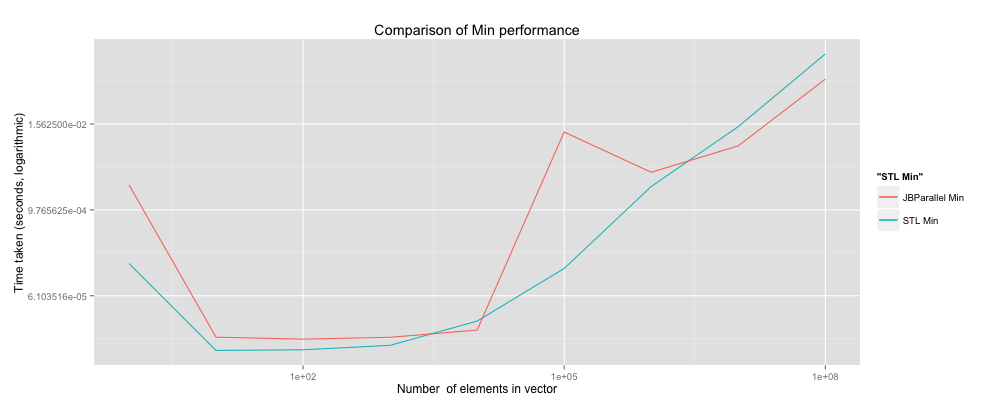
\includegraphics[scale = 0.4]{Min_comparison}
    \caption{\textbf{Performance on min\_element}:\\We see that as the number of elements increases, our code begins. Fluctuations likely due to randomness (code too slow to run for a lot of trials)}
    \end{figure}
 \begin{figure}[h!]
    \centering
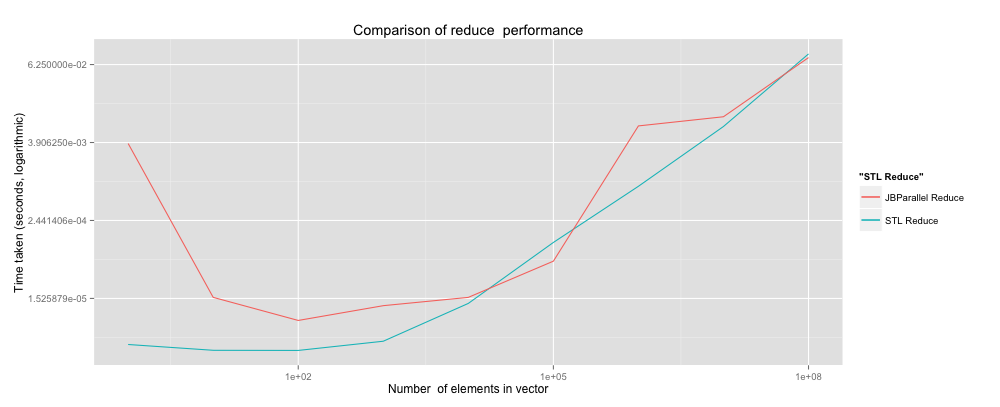
\includegraphics[scale = 0.4]{Reduce_comparison}
    \caption{\textbf{Performance on reduce}:\\ Our code begins to outperform a serial reduction loop at about the $4 \times 10^6$ element mark, up to an ultimate speedup of about 2.0x.  Same causes for randomness as above.}
    \end{figure}
     \begin{figure}[h!]
    \centering
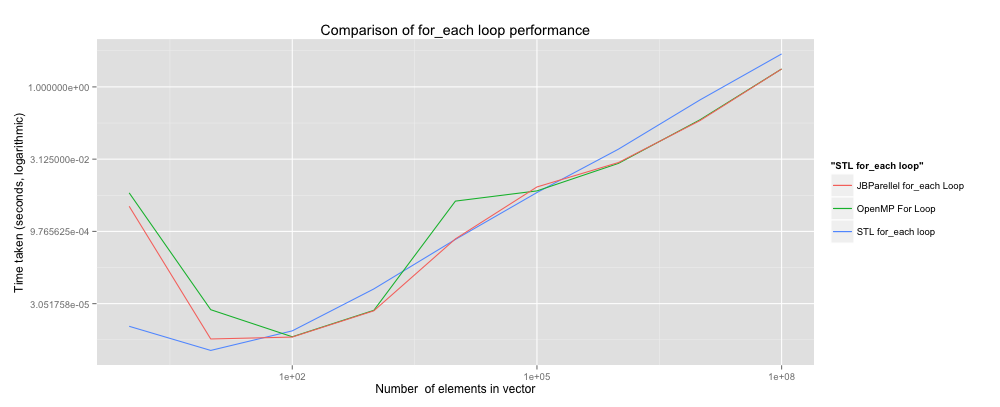
\includegraphics[scale = 0.4]{for_each_loop_comparison}
    \caption{\textbf{Performance on for\_each}:\\ Code begins to outperform at around the million element mark. It also consistently outperforms OpenMP on large problem sizes by about 1.2x Same causes for randomness  as above.}
    \end{figure}
     \begin{figure}[h!]
    \centering
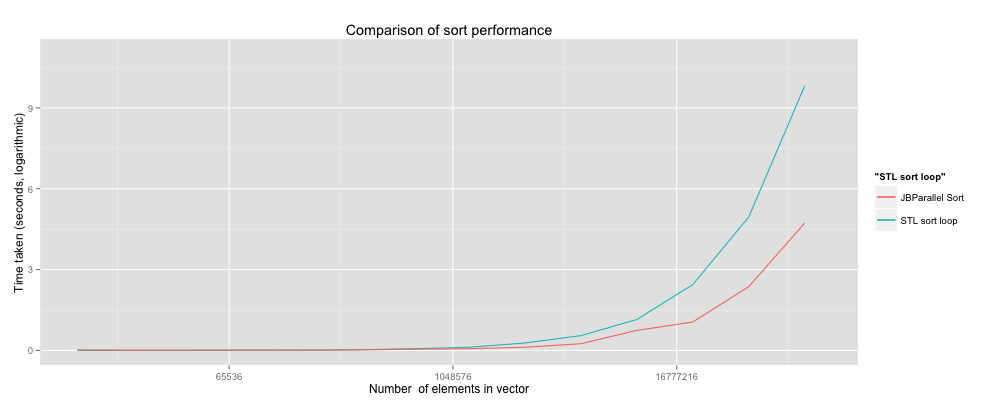
\includegraphics[scale = 0.4]{sort_comparison}
    \caption{\textbf{Performance on sort}:\\ Again we win at large sizes, same causes for randomness as above.}
    \end{figure}
 \newpage

		\begin{figure}[t!]
		\centering
		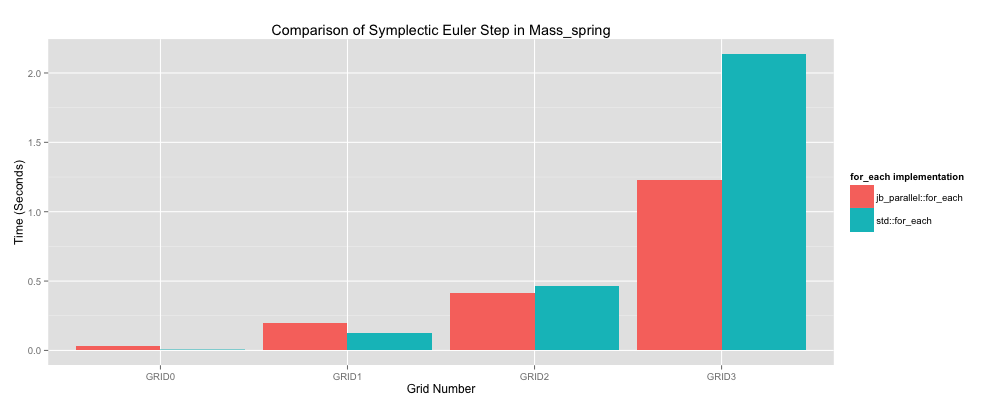
\includegraphics[scale = 0.4]{symplectic_comparison}
		\caption{\textbf{Performance on symplectic\_euler\_step in mass\_spring.cpp}:\\ We win for larger graph sizes, but still overhead in small grids.}
		\end{figure}


It's important to note that in each of these figures, very little work is being done on each iteration of the parallel/non-parallel loop.  The more work done on each iteration, however, the more the parallel algorithm wins, so in general practice, one would expect more speedup than is shown here.  Other interesting results we came across while working on things in a test environment: nesting a parallel loop within non-parallel loops is very, very costly (unfortunately this is inevitable on the *step functions because we can't really compute things in the future), and using shared variables via OpenMP's \texttt{shared} keyword.

Here is a typical run of our testing file, ptest.cpp, which is in our project directory.

\begin{verbatim}
Min element found by serial: 0
Serial Min: 0.0878805s
Min element found by parallel: 0
jb_parallel parallel_min: 0.0462203s

Serial Parallel Loop: 2.64941s
OMP Parallel Loop: 1.05172s
JB Parallel_Transform: 0.480762s

Serial Sort: 2.30043s
Parallel Sort: 0.930822s

Serial reduction: 0.0699698s
0
Parallel reduction: 0.0174481s
0
\end{verbatim}

To run this inside our repo and get similar results, simply run \texttt{make ptest}, followed by \texttt{./ptest}.

As you can see, this run was slightly atypical in terms of speed, but in line with the numbers stated above.  We found that speed data was difficult to collect consistently, so we wrote speedtest.py to allow us to run our code easily hundreds or thousands of times (typically we would see acceleration after multiple runs, probably due to some sort of caching issue).  Of course the issue there was that in order to see speedup, we needed to be working with large amounts of data, but then the task would take long enough that running the code say, a thousand times would become impractical

Another tool which assisted us enormously in our quest to make code fast was valgrind's callgrind profiler tool, and kcachegrind, a tool which provides a GUI to visualize callgrind output.  For example, in speeding up George's code (they used our extension and sped their code up, and we used our extension and sped their code up in parallel :)), we first ran:

\begin{verbatim}
valgrind --tool=callgrind ./mesh_mass_spring data/sphere2.nodes data/sphere2.tris
\end{verbatim}

The program kcachegrind allows one to see the output of this profiler using a nice GUI which allows for visualization of the call graph, call map, and raw call counts for all functions, which is extremely helpful in profiling.  We found in George's code that the mesh\_shape\_volume function was particularly slow, and was also a great use case of parallel\_reducer, so we used this to achieve about 2x speed up (this will only work with very large inputs). 



\section{Collaboration Evaluations}

The extensions provided by other students on Piazza was invaluable to our project. We were given large amounts of very well written C++ code that included for\_loops that could be easily parallelized using our jb\_parallel library.  Note that for all of these, we only looked at a specific subset of the code in the hopes of optimizing it.  Also please take any criticisms we have with a grain of salt, as we often grabbed code from these projects while they were still in an intermediate state, and this probably accounts for any problems we had.


\subsection{George Lok and Serguei Balanovich}

Very well written, understandable code.  We really liked the way their code was laid out.  This allowed us to quickly, and modularly, modify their code.  And we understand they used our package as well, independently of us!

\subsection{Brian Zhang and Tarik Moon}

At the time we received it, the code wasn't super well documented, lots of stuff un-commented and lots of stuff commented out.  Again, we think we just received the code at an unfavorable time, when that group was still figuring stuff out (because we could pull after any commit).  Nonetheless, we were extremely impressed with the results of the project.

\subsection{Wenshuai Ye and Yuhao Zhu}

Nice implementation of mesh, very fast, but lots of compiler warnings, some of which were removed, but not all.

Wenshuai and Yuhao wrote a great extension to shallow\_water called shallow\_water\_extension.cpp. We also used their Mesh.cpp file, which we renamed Mesh2.cpp to not conflict with our existing code. 

In Mesh2.cpp, we rewrote their triangle\_iterator to make it a Random Access Iterator.

In shallow\_water\_extension.cpp, we refactored the code inside of the hyperbolic\_step to create a functor called FluxUpdater with the exact same logic as before. This allowed us to use their code in our jb\_parallel::for\_each, which parallelized their code.

%\subsection{Erik and Lukas}
%Code was spread across (too) many files, which made things a bit difficult.  Also .  Ended up

\end{document}
